%
% design.tex
%
% Copyright (C) 2022 by SpaceLab.
%
% OBDH 2.0 Module
%
% This work is licensed under the Creative Commons Attribution-ShareAlike 4.0
% International License. To view a copy of this license,
% visit http://creativecommons.org/licenses/by-sa/4.0/.
%

%
% \brief Design slides.
%
% \author Gabriel Mariano Marcelino <gabriel.mm8@gmail.com>
% \author Bruno Benedetti <brunobenedetti45@gmail.com>
%
% \version 0.1.0
%
% \date 2022/07/28
%


\begin{frame}{Specifications}

    \begin{itemize}
        \item Microcontroller: MSP430F6659/MSP430F5659
        \item Clock: 32 MHz
        \item Memories:
        \begin{itemize}
            \item RAM: 64 kB (SRAM)
            \item Flash: 512 kB (code), 1 Gb NOR (mass storage)
            \item FRAM: 2 Mb
        \end{itemize}
        \item Sensors: Voltage, current and temperature
        \item Interfaces: UART, I$^{2}$C, SPI, GPIO, PWM, ADC, DAC and RS-485
        \item Mass: 53 g
        \item PC-104 compatible
    \end{itemize}

\end{frame}

% #########################################################################
% #########################################################################

\begin{frame}{Electrical Block Diagram}

    \begin{figure}[!ht]
        \begin{center}
            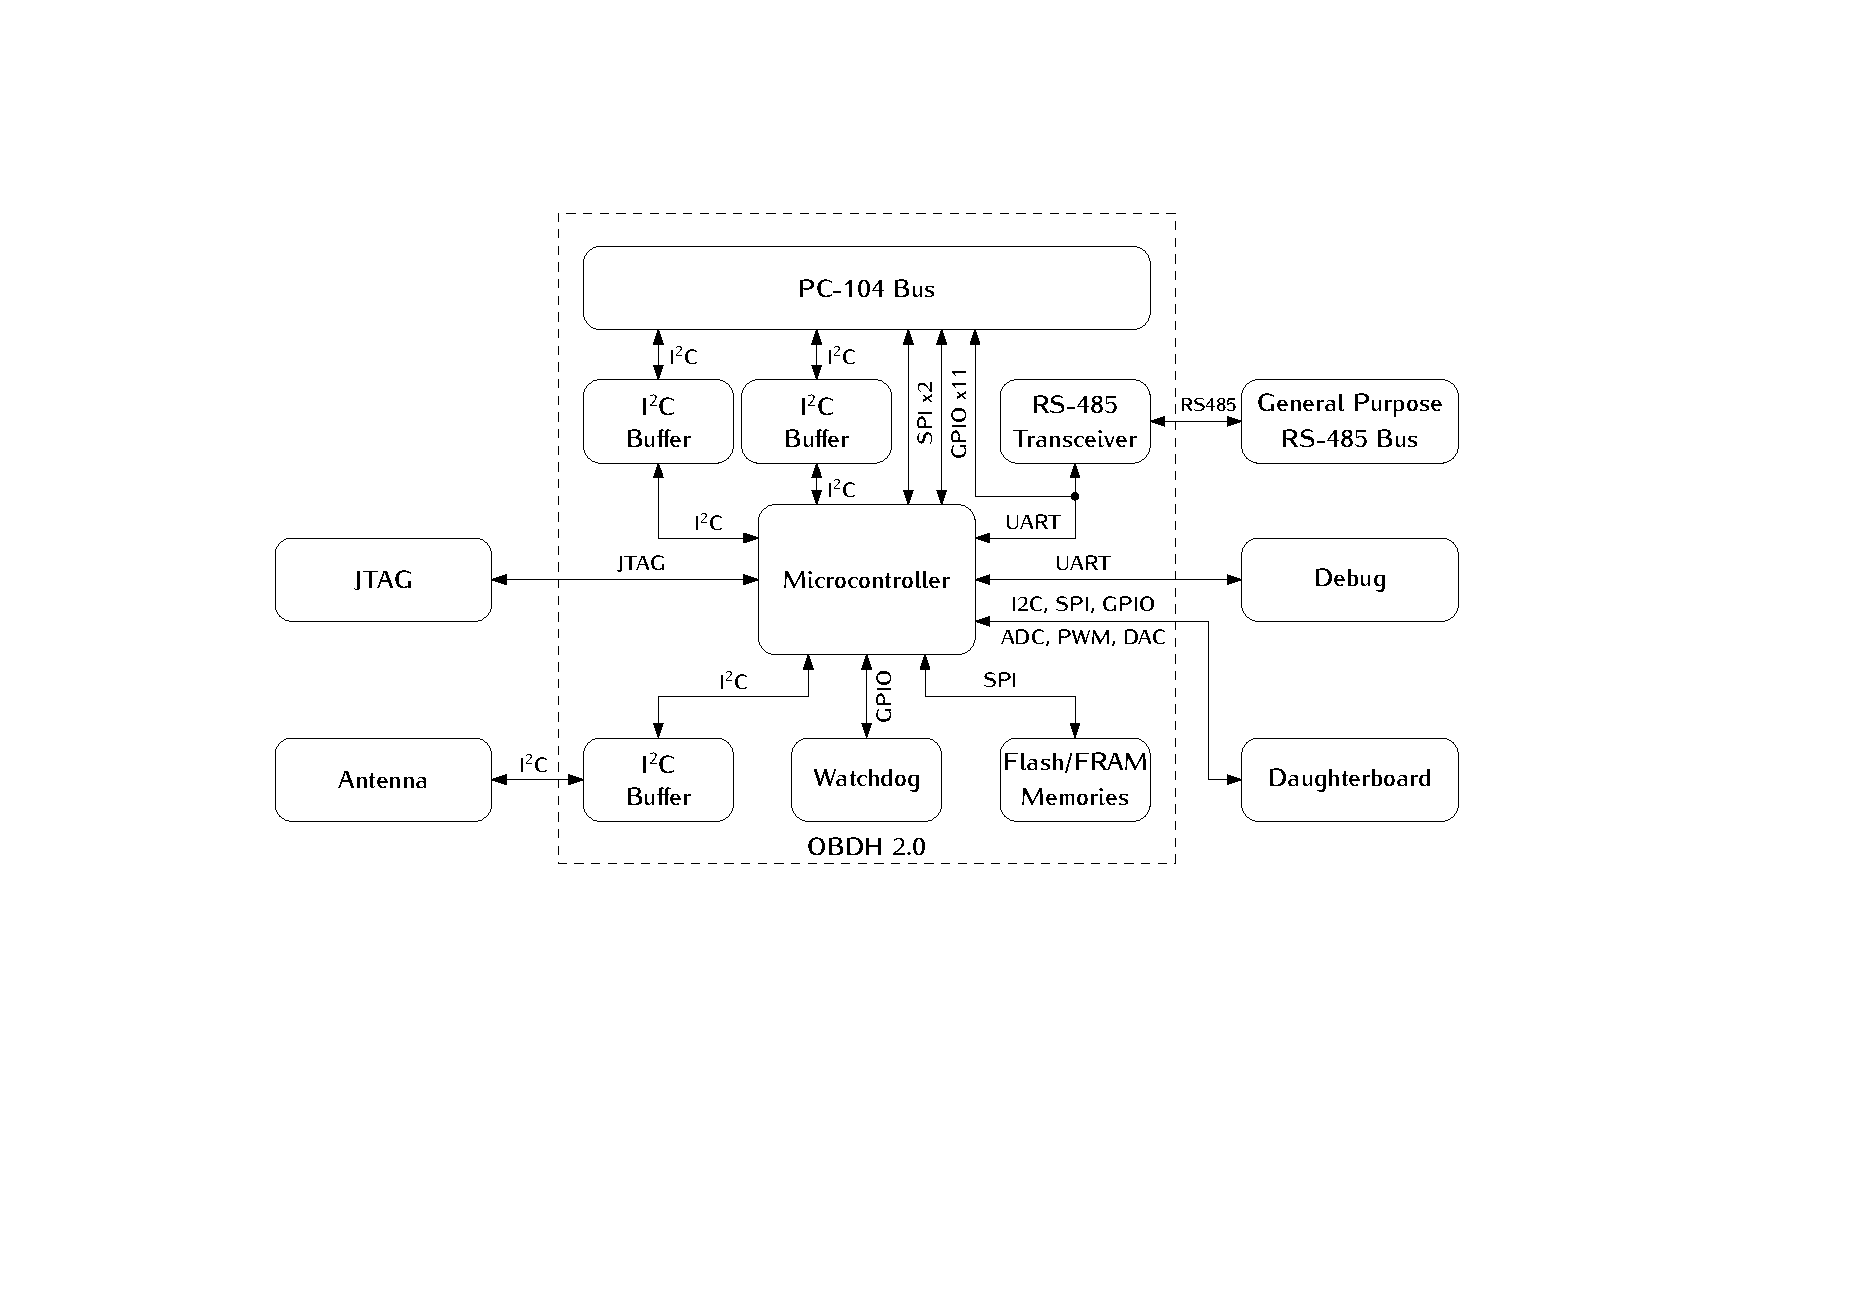
\includegraphics[width=11cm]{figures/block-diagram}
        \end{center}
    \end{figure}

\end{frame}

\begin{frame}{Schematics}

    Available at: \href{https://github.com/spacelab-ufsc/obdh2/tree/master/hardware/outputs/board_schematics}{\textcolor{blue}{\underline{https://github.com/spacelab-ufsc/obdh2}}}

    \begin{figure}[!ht]
        \begin{center}
            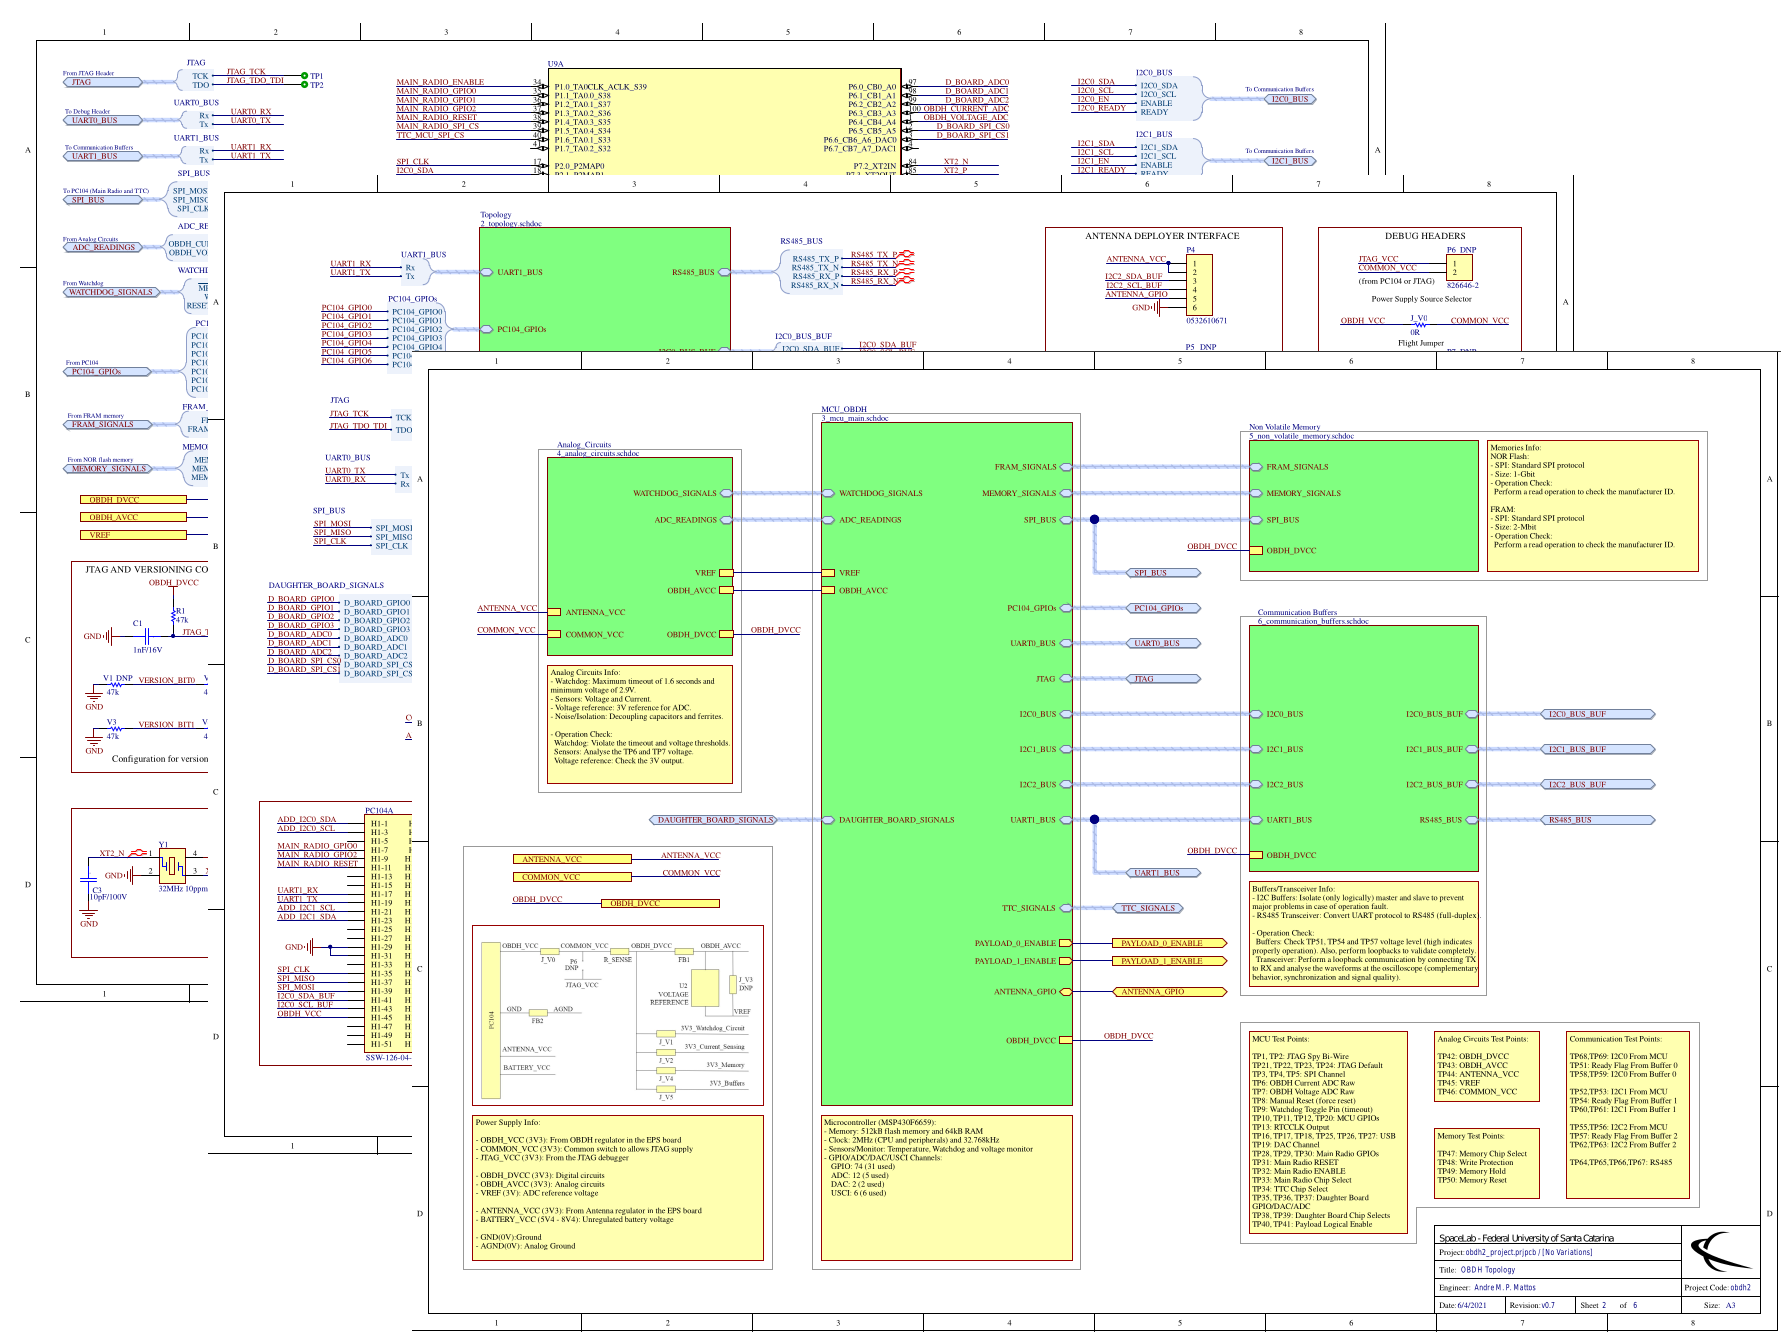
\includegraphics[width=8.5cm]{figures/obdh2-schematics.png}
        \end{center}
    \end{figure}

\end{frame}

\begin{frame}{PCB Layout}

    Available at: \href{https://github.com/spacelab-ufsc/obdh2/tree/master/hardware/sources}{\textcolor{blue}{\underline{https://github.com/spacelab-ufsc/obdh2}}}

    \begin{columns}[t]
        \begin{column}[t]{0.5\textwidth}
            \begin{figure}[!ht]
                \begin{center}
                    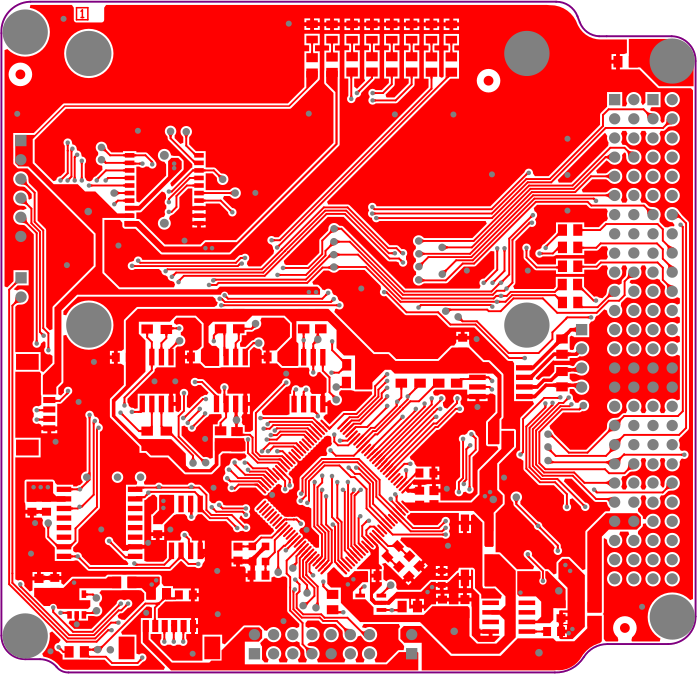
\includegraphics[width=5cm]{figures/obdh2-layout-top.png}
                \end{center}
                \caption{Top side}
            \end{figure}
        \end{column}
        \begin{column}[t]{0.5\textwidth}
            \begin{figure}[!ht]
                \begin{center}
                    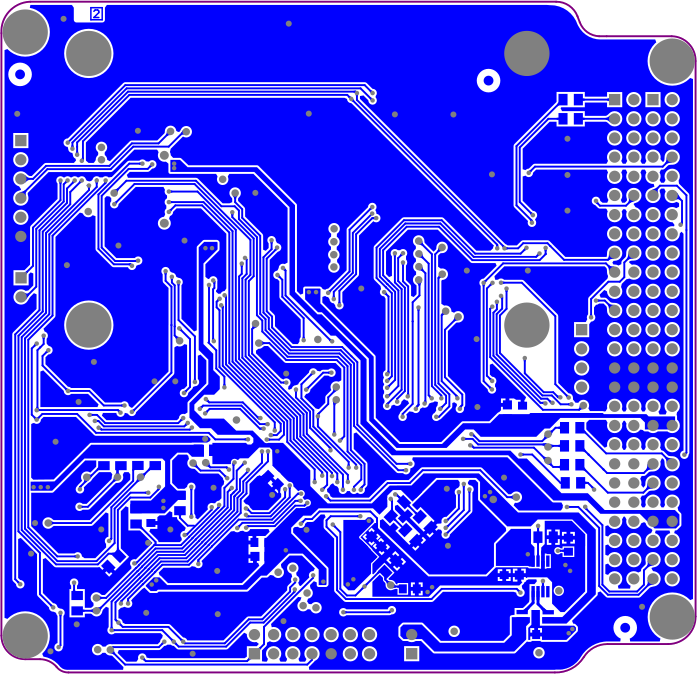
\includegraphics[width=5cm]{figures/obdh2-layout-bottom.png}
                \end{center}
                \caption{Bottom side}
            \end{figure}
        \end{column}
    \end{columns}

\end{frame}

\begin{frame}{3D Model}

    Available at: \href{https://github.com/spacelab-ufsc/obdh2/tree/master/hardware/outputs/board_3dmodels}{\textcolor{blue}{\underline{https://github.com/spacelab-ufsc/obdh2}}}

    \begin{figure}[!ht]
        \begin{center}
            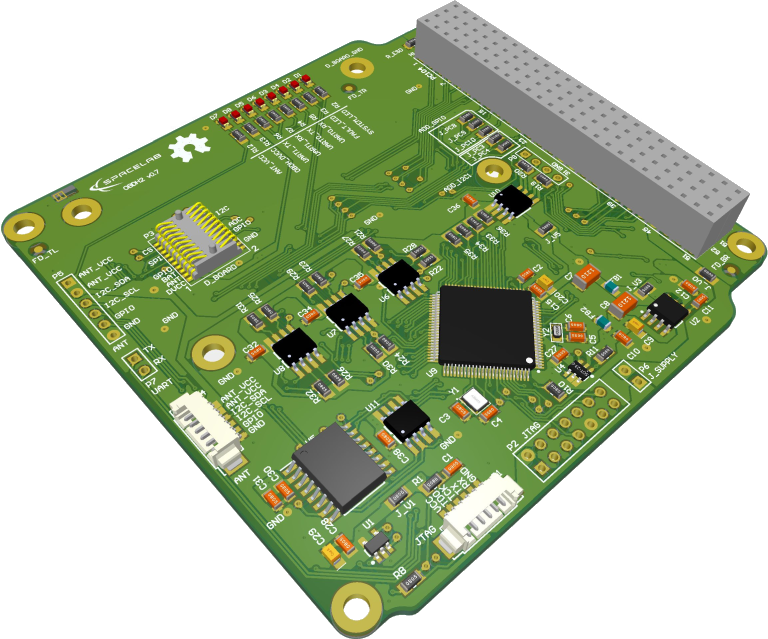
\includegraphics[width=7.5cm]{figures/obdh2-pcb-3d.png}
        \end{center}
    \end{figure}

\end{frame}

% #########################################################################
% #########################################################################

\begin{frame}{Power Consumption}

    \begin{itemize}
        \item Normal operation $\cong$ \textbf{66 mW} (3,3 V @ 20 mA) 
    \end{itemize}

    \begin{figure}[!ht]
        \begin{center}
            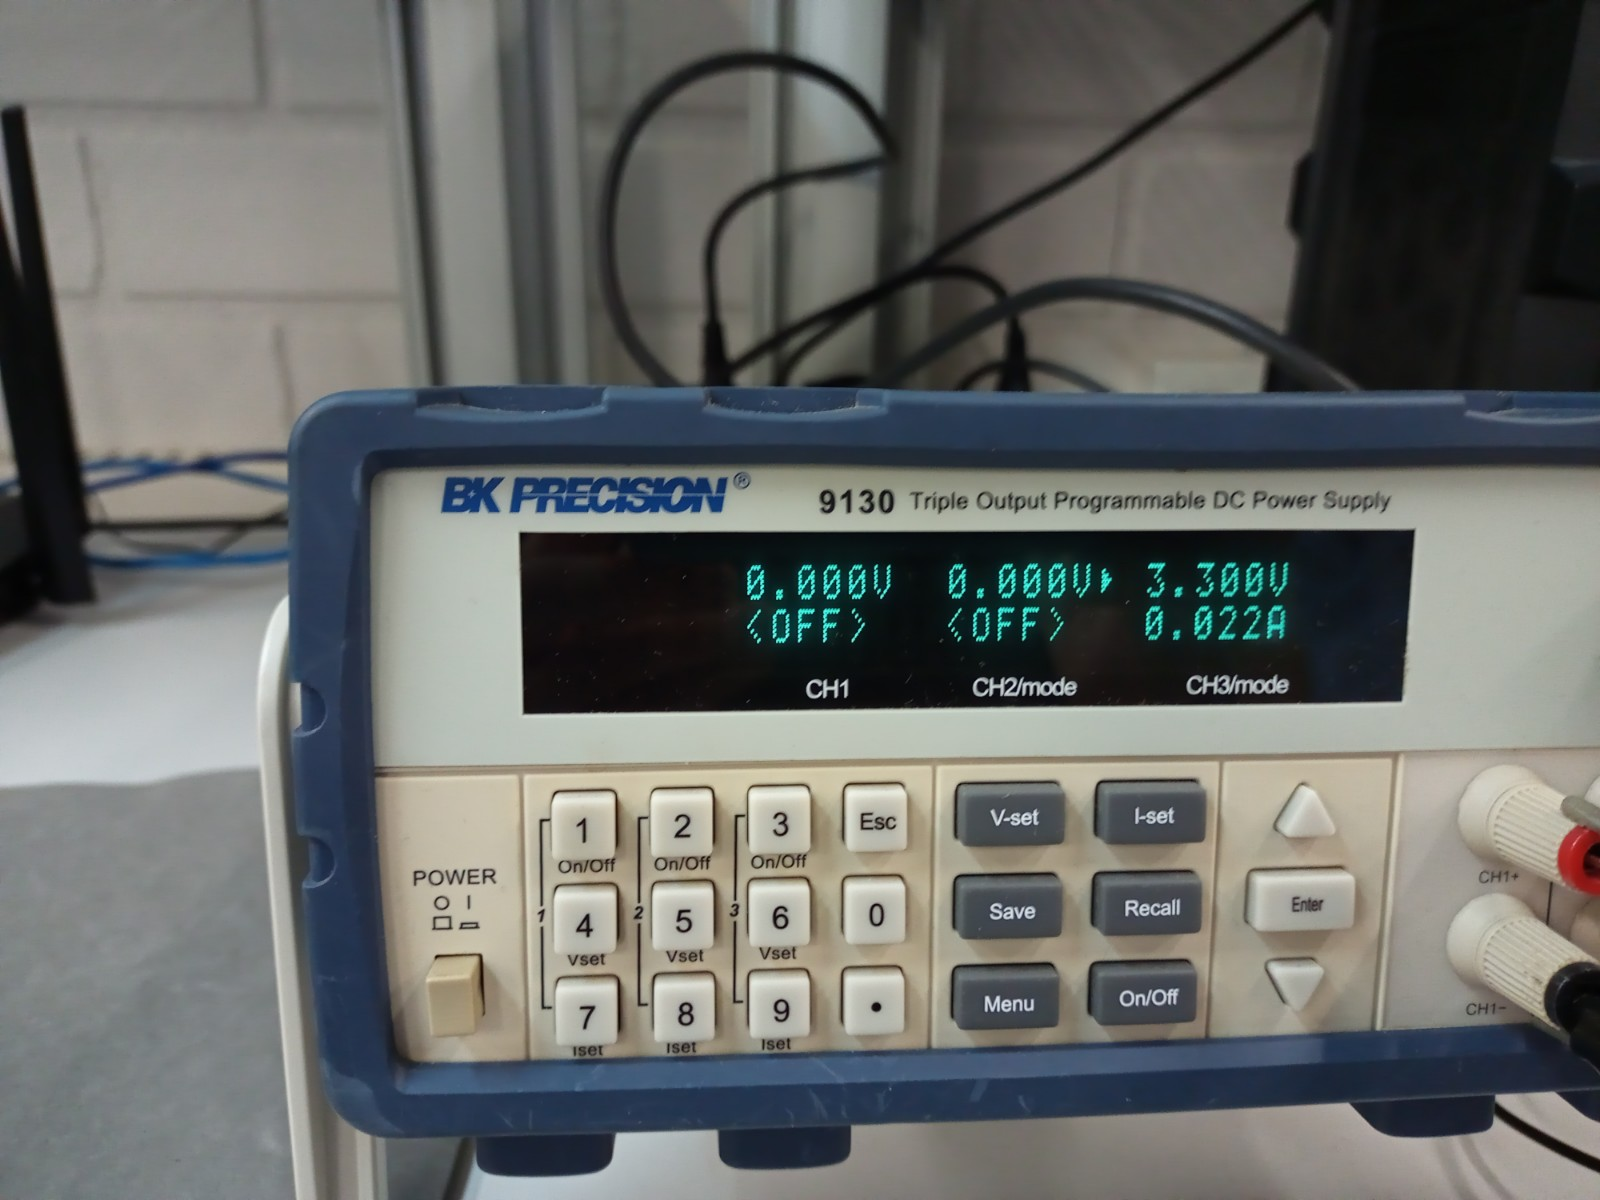
\includegraphics[width=7.5cm]{figures/obdh2-consumption.jpg}
        \end{center}
    \end{figure}

\end{frame}

% #########################################################################
% #########################################################################

\begin{frame}{Electrical Interfaces: PC-104}

\begin{table}[!h]\tiny
    \centering
    \begin{tabular}{cllll}
        \toprule[1.5pt]
        \textbf{Pin [A-B]} & \textbf{H1A}     & \textbf{H1B}     & \textbf{H2A}  & \textbf{H2B}  \\
        \midrule
        1-2                & -                & -                & -             & -             \\
        3-4                & -                & -                & GPIO\_4       & GPIO\_5       \\
        5-6                & -                & -                & -             & -             \\
        7-8                & GPIO\_0          & GPIO\_1          & -             & GPIO\_6       \\
        9-10               & GPIO\_2          & -                & -             & -             \\
        11-12              & GPIO\_3          & GPIO\_7          & SPI\_0\_MOSI  & SPI\_0\_CLK   \\
        13-14              & -                & -                & SPI\_0\_CS\_1 & SPI\_0\_MISO  \\
        15-16              & -                & -                & -             & -             \\
        17-18              & UART\_1\_RX      & GPIO\_8          & -             & -             \\
        19-20              & UART\_1\_TX      & GPIO\_9          & -             & -             \\
        21-22              & -                & -                & -             & -             \\
        23-24              & -                & -                & -             & -             \\
        25-26              & -                & -                & -             & -             \\
        27-28              & -                & -                & -             & -             \\
        29-30              & GND              & GND              & GND           & GND           \\
        31-32              & GND              & GND              & GND           & GND           \\
        33-34              & -                & -                & -             & -             \\
        35-36              & SPI\_0\_CLK      & -                & VCC\_3V3\_ANT & VCC\_3V3\_ANT \\
        37-38              & SPI\_0\_MISO     & -                & -             & -             \\
        39-40              & SPI\_0\_MOSI     & SPI\_0\_CS\_0    & -             & -             \\
        41-42              & I2C\_0\_SDA      & -                & -             & -             \\
        43-44              & I2C\_0\_SCL      & -                & -             & -             \\
        45-46              & VCC\_3V3         & VCC\_3V3         & VCC\_BAT      & VCC\_BAT      \\
        47-48              & -                & -                & -             & -             \\
        49-50              & -                & -                & I2C\_1\_SDA   & -             \\
        51-52              & -                & -                & I2C\_1\_SCL   & -             \\
        \bottomrule[1.5pt]
    \end{tabular}
    \label{tab:pc104-pins}
\end{table}

\end{frame}

\begin{frame}{Other Electrical Interfaces}

    \begin{table}[!htb]\tiny
        \centering
        \begin{tabular}{cccl}
            \toprule[1.5pt]
            \textbf{Connector} & \textbf{Interface} & \textbf{Type} & \textbf{Pins} \\
            \midrule
            \multirow{6}{*}{P1}  & \multirow{6}{*}{JTAG}  & \multirow{6}{*}{PicoBlade}   & VCC\_3V3 \\
                                 &                        &                              & TDO\_TDI \\
                                 &                        &                              & TCK \\
                                 &                        &                              & UART\_TX \\
                                 &                        &                              & UART\_RX \\
                                 &                        &                              & GND \\
            \midrule
            \multirow{14}{*}{P2} & \multirow{14}{*}{JTAG} & \multirow{14}{*}{Pin Header} & TDO\_TDI \\
                                 &                        &                              & VCC\_3V3 \\
                                 &                        &                              & None \\
                                 &                        &                              & None \\
                                 &                        &                              & None \\
                                 &                        &                              & None \\
                                 &                        &                              & TCK \\
                                 &                        &                              & None \\
                                 &                        &                              & GND \\
                                 &                        &                              & None \\
                                 &                        &                              & None \\
                                 &                        &                              & UART\_TX \\
                                 &                        &                              & None \\
                                 &                        &                              & UART\_RX \\
            
            \bottomrule[1.5pt]
        \end{tabular}
    \end{table}

\end{frame}

\begin{frame}{Other Electrical Interfaces}

    \begin{table}[!htb]\tiny
        \centering
        \begin{tabular}{cccll}
            \toprule[1.5pt]
            \multirow{2}{*}{\textbf{Connector}} & \multirow{2}{*}{\textbf{Interface}} & \multirow{2}{*}{\textbf{Type}} & \multicolumn{2}{c}{\textbf{Pins}} \\
                                                &                                     &                                & \textbf{Row A} & \textbf{Row B} \\
            \midrule
            \multirow{10}{*}{P3} & \multirow{10}{*}{Daughterboard} & \multirow{10}{*}{DSI} & VCC\_3V3       & GND \\
                                 &                                 &                       & VCC\_3V3\_ANT  & GND \\
                                 &                                 &                       & VCC\_BAT       & GND \\
                                 &                                 &                       & GPIO\_0        & GPIO\_1\\
                                 &                                 &                       & GPIO\_2        & GPIO\_3\\
                                 &                                 &                       & SPI\_0\_CLK    & ADC\_0 \\
                                 &                                 &                       & SPI\_0\_MISO   & ADC\_1 \\
                                 &                                 &                       & SPI\_0\_MOSI   & ADC\_2 \\
                                 &                                 &                       & SPI\_0\_CS\_0  & I2C\_2\_SDA \\
                                 &                                 &                       & SPI\_0\_CS\_1  & I2C\_2\_SCL \\
            \bottomrule[1.5pt]
        \end{tabular}
    \end{table}

\end{frame}

\begin{frame}{Other Electrical Interfaces}

    \begin{table}[!htb]\tiny
        \centering
        \begin{tabular}{cccl}
            \toprule[1.5pt]
            \textbf{Connector} & \textbf{Interface} & \textbf{Type} & \textbf{Pins}\\
            \midrule
            \multirow{6}{*}{P4} & \multirow{6}{*}{I2C} & \multirow{6}{*}{PicoBlade}  & VCC\_3V3\_ANT \\
                                &                       &                             & VCC\_3V3\_ANT \\
                                &                       &                             & I2C\_SDA \\
                                &                       &                             & I2C\_SCL \\
                                &                       &                             & GPIO \\
                                &                       &                             & GND \\
            \midrule
            \multirow{6}{*}{P5} & \multirow{6}{*}{I2C} & \multirow{6}{*}{Pin Header} & VCC\_3V3\_ANT \\
                                &                       &                             & VCC\_3V3\_ANT \\
                                &                       &                             & I2C\_SDA \\
                                &                       &                             & I2C\_SCL \\
                                &                       &                             & GPIO \\
                                &                       &                             & GND \\
            \midrule
            \multirow{2}{*}{P6} & \multirow{2}{*}{Power} & \multirow{2}{*}{Pin Header} & JTAG\_VCC \\
                                &                       &                                    & COMMOM\_VCC \\
            \midrule
            \multirow{2}{*}{P7} & \multirow{2}{*}{UART} & \multirow{2}{*}{Pin Header} & UART\_TX \\
                                &                       &                             & UART\_RX \\
            \midrule
            \multirow{4}{*}{P8} & \multirow{4}{*}{RS-485} & \multirow{4}{*}{Pin Header} & RS485\_RX +\\
                                &                       &                               & RS485\_RX -\\
                                &                       &                               & RS485\_TX -\\
                                &                       &                               & RS485\_TX +\\
            \bottomrule[1.5pt]
        \end{tabular}
    \end{table}

\end{frame}

\begin{frame}{Dimensions}

    \begin{figure}[!ht]
        \begin{center}
            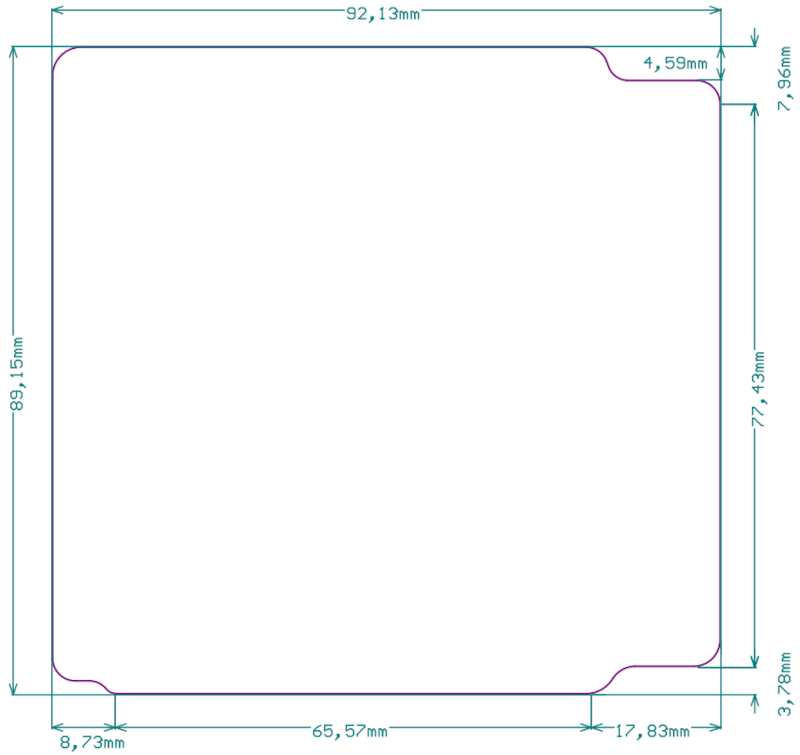
\includegraphics[width=7.5cm]{figures/board-dimensions.png}
        \end{center}
    \end{figure}

\end{frame}

\begin{frame}{External Memories}

    \begin{table}[!htb]
        \centering
        \begin{tabular}{lcc}
            \toprule[1.5pt]
            \textbf{Characteristic} & \textbf{Flash NOR} & \textbf{FRAM} \\
            \midrule
            Manufacturer      & Micron                 & Cypress \\
            Partnumber        & MT25QL01GBBB           & CY15B102QN \\
            Capacity          & 128 MB                 & 2 Mb \\
            Erase cycles      & $10^{5}$               & $10^{13}$ \\
            Data retention    & 2 years                & 121 years \\
            Interface         & SPI                    & SPI \\
            Temperature range & -40 to 125 $^{\circ}$C & -40 to 125 $^{\circ}$C \\
            \bottomrule[1.5pt]
        \end{tabular}
    \end{table}

\end{frame}

\begin{frame}{Sensors}

    \begin{itemize}
        \item Current sensor: MAX9934
        \vspace{0.3cm}
        \item Voltage sensor: TLV341A
        \vspace{0.3cm}
        \item Temperature sensor: $\mu$C (internal sensor)
        \vspace{0.3cm}
    \end{itemize}

\end{frame}

\begin{frame}{External Watchdog}

    \begin{itemize}
        \item IC: Texas Instruments TPS3823
        \vspace{0.5cm}
        \item Voltage monitor with a watchdog timer feature
        \vspace{0.5cm}
        \item Timeout period: $1600\ ms$
        \vspace{0.5cm}
        \item Reset period: $100\ ms$
    \end{itemize}

\end{frame}

\begin{frame}{Daughterboard}

    \begin{figure}[!ht]
        \begin{center}
            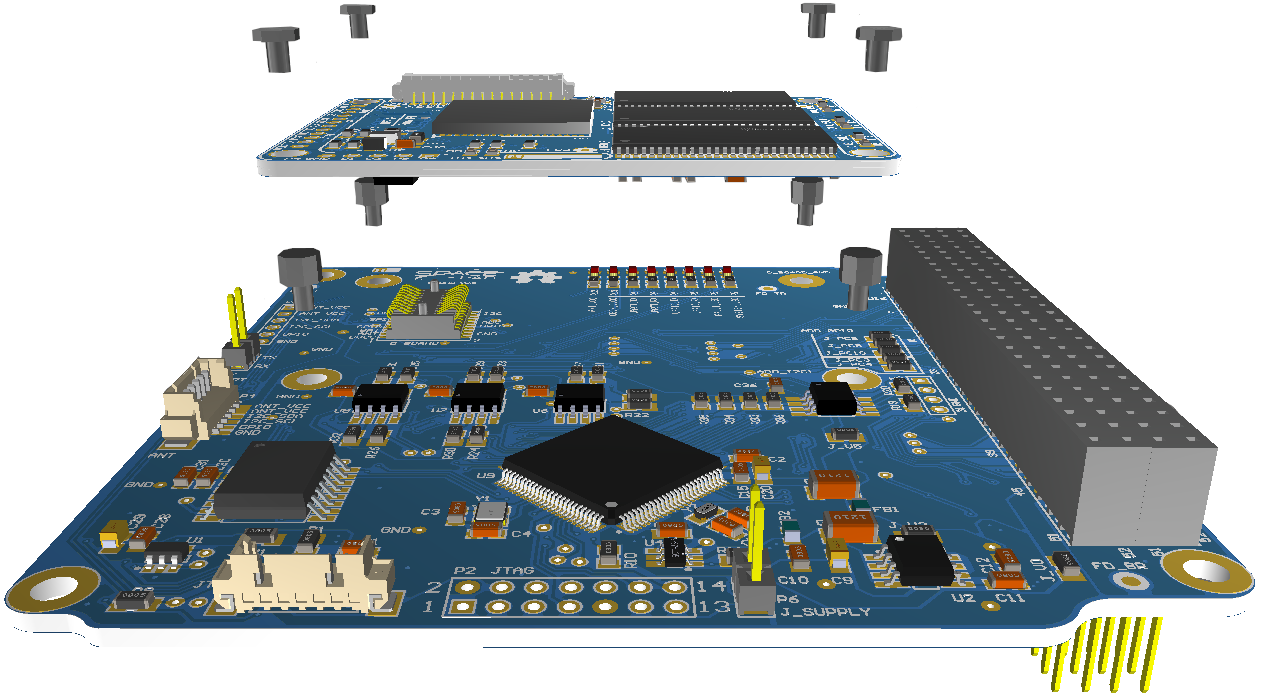
\includegraphics[width=9cm]{figures/daughterboard-integration.png}
        \end{center}
    \end{figure}

\end{frame}

\begin{frame}{Flight Model Specs. and Preparation}

    \begin{itemize}
        \item PCB specs.: IPC 6012 Class 3
        \vspace{0.3cm}
        \item PCB thickness: 1,6 mm
        \vspace{0.3cm}
        \item Material: TG170 FR-4
        \vspace{0.3cm}
        \item Surface finish: ENIG
        \vspace{0.3cm}
        \item Conformal coating application
    \end{itemize}

\end{frame}